\documentclass[border=4pt]{standalone}
\usepackage{tikz}
\usetikzlibrary{matrix, positioning, arrows.meta}
\usepackage{xcolor}
\usepackage{amsmath, amssymb}
\definecolor{accent}{RGB}{195,30,55}
\definecolor{cool}{RGB}{31,120,180}
\newcommand{\pia}{\pi_{\alpha}}
\newcommand{\sigxi}{\sigma_{\xi}}
\newcommand{\siga}{\sigma_{\alpha}}
\newcommand{\sigr}{\sigma_{r}}
\newcommand{\sigz}{\sigma_{\zeta}}
\newcommand{\siglam}{\sigma_{\lambda}}
\newcommand{\sigs}{\sigma_{s}}
\newcommand{\kappap}{\kappa_{\text{pop}}}
\begin{document}
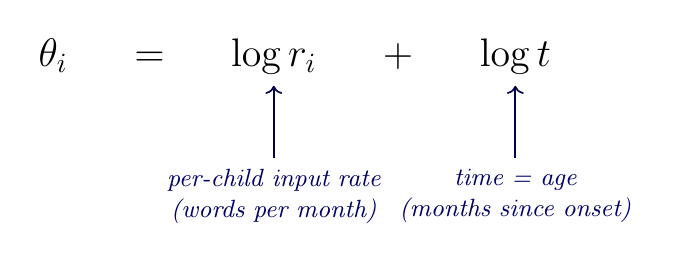
\begin{tikzpicture}[
  every node/.style={inner sep=2pt},
  ann/.style={font=\small\itshape, color=blue!40!black,
              align=center, text width=3.5cm},
  arrow/.style={->, blue!30!black, semithick, shorten >=2pt, shorten <=2pt}]
\matrix[matrix of nodes, column sep=20pt, nodes={font=\Large},
        ampersand replacement=\&]{
  |[name=t1]| $\theta_i$ \&
  $=$ \&
  |[name=logr]| $\log r_i$ \&
  $+$ \&
  |[name=logt]| $\log t$ \\
};
\node[ann, below=3em of logr] (alogr)
  {per-child input rate\\(words per month)};
\draw[arrow] (alogr) -- (logr);
\node[ann, below=3em of logt] (alogt)
  {time = age\\(months since onset)};
\draw[arrow] (alogt) -- (logt);
\end{tikzpicture}
\end{document}
